\newpage
\usecaseristoratore{Visualizzazione notifica di inserimento \textit{feedback}}
\label{usecase:Visualizzazione notifica di inserimento feedback}

\begin{figure}[h]
	\centering
	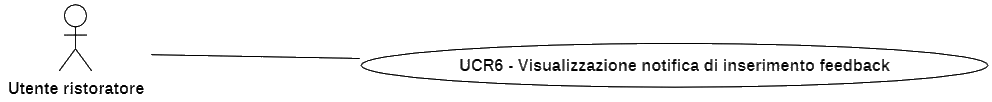
\includegraphics[width=0.9\textwidth]{./uml/UCR6.png} 
	\caption{Visualizzazione notifica di inserimento \textit{feedback}}
	\label{fig:UCR6}
  \end{figure}

\begin{itemize}
	\item \textbf{Attore principale:} Utente ristoratore.

	\item \textbf{Precondizione:} L'Utente base ha confermato l'inserimento del \textit{feedback} (vedi \autoref{usecase:Inserimento di feedback e recensioni}).

	\item \textbf{Postcondizione:} L'Utente ristoratore visualizza la notifica dell'inserimento di un \textit{feedback} da parte del cliente.

	\item \textbf{Scenario principale:}
	      \begin{enumerate}
		      \item Il Sistema vede che al suo interno è stata inserita una nuova recensione;
		      \item Il Sistema invia al ristoratore la notifica relativa all'inserimento di una recensione;
		      \item L'Utente ristoratore visualizza la notifica dell'inserimento di un \textit{feedback} da parte del cliente.
	      \end{enumerate}
\end{itemize}
